\documentclass{beamer}
\usepackage[utf8x]{inputenc}
\usepackage[english, russian]{babel}
\usepackage{amsmath}
\usepackage{graphicx}
\usetheme{Boadilla}
\title{Задача 6.9}
\author{Огородников Д.М., Васильченко Д.Д.}
\institute{МГУ им. М.В. Ломоносова}

\begin{document}
	
\begin{frame}
	\titlepage	
\end{frame}
\begin{frame}
	\frametitle{Постановка задача}
	Одномерная цепочка чередующихся атомов разной массой $m$ и $M$. Соединены пружинами одинаковой жесткости $\beta$ и длины $l$ \newline
	Вывести уравнение движения масс. Получить дисперсионное соотношение $\omega = \omega(k)$ и построить соотвествующие графики для акустической и оптической ветвей дисперсионной кривой.
\end{frame}
\begin{frame}
	\frametitle{Решение}
	Обозначим смещения $\eta_n$  и $\xi_n$. Рассмотрим внешние силы взаимодействия только соседних атомов.
	\begin{equation*}
		\begin{cases}
			M \ddot{\xi_n} = \beta (\eta_n - 2\xi_n + \eta_{n+1}) \\
			m \ddot{\eta_n} = \beta(\xi_{n-1} - 2\eta_n + \xi_n)
		\end{cases}
	\end{equation*}
	Будем искать частное решение в виде бегущих волн:
	\begin{equation*}
		\begin{cases}	
			\xi_n = \xi_0 e^{i(\omega t - kb}) \\
			\eta_n = \eta_0 e^{i(\omega t - kb + \frac{kb}{2})},  k \in [-\frac\pi{b}, \frac\pi{b}]
		\end{cases}	
	\end{equation*}
\end{frame}
\begin{frame}
	Подставляем
	\begin{equation*}
		\begin{cases}
			(M \omega^2 - 2 \beta) \xi_0 + \beta (e^{\frac{ikb}{2}} - e^{-\frac{ikb}{2}}) \eta_0 = 0 \\
			\beta (e^{\frac{ikb}{2}} - e^{-\frac{ikb}{2}}) \xi_0 + (m\omega^2 - 2 \beta) \eta_0 = 0
		\end{cases}
	\end{equation*}
	Рассмотрим уравнение для коэффициентов $det A = 0$
	\begin{equation*}
		Mm\omega^4 -2 \beta (M + m) \omega^2 + 2 \beta^2 (1 - \cos{kb}) = 0	
	\end{equation*}
	Решение имеет вид: 
	\begin{equation*}
		\omega^2 = \frac{\beta}{Mm} \left(M + m \pm \sqrt{M^2 + m^2 + 2 M m \cos{kb}}\right)
	\end{equation*}

\end{frame}
\begin{frame}
	Рассмотрим случай $M = m$, тогда
	\begin{equation*}
		\omega^2 = \frac{2\beta}{m} (1 \pm \cos{\frac{kb}{2}})
	\end{equation*}
	$$
		\omega_{+} = 2\sqrt{\frac{\beta}{m}} \cos{\frac{kb}{4}}
	$$
	$$
		\omega_{-} = 2\sqrt{\frac{\beta}{m}} \sin{\frac{kb}{4}}
	$$
	\begin{figure}[ht!]
		\centering
		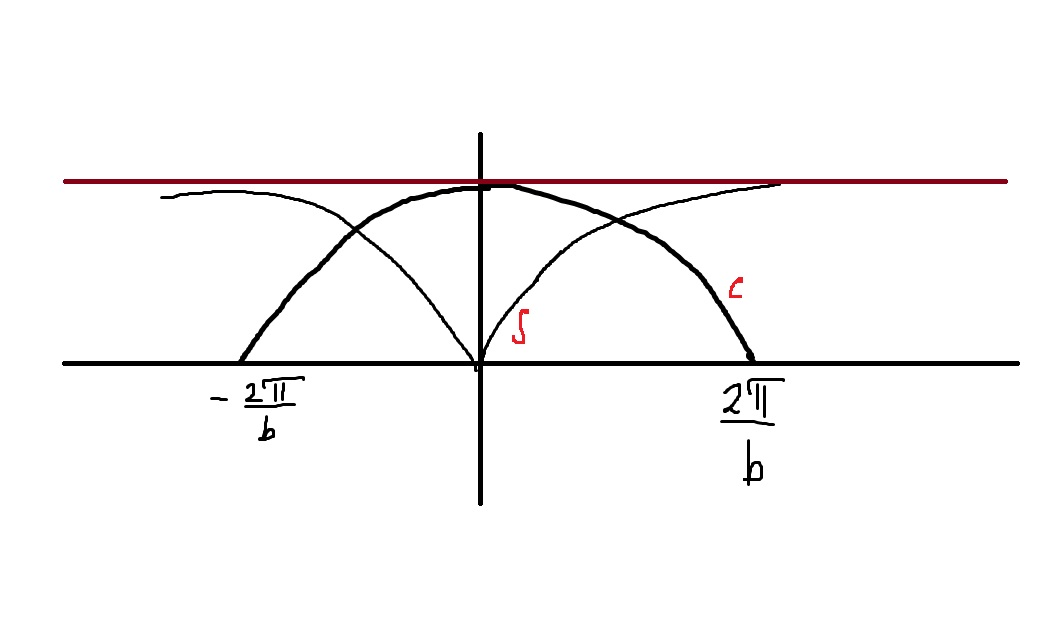
\includegraphics[width=90mm]{1.jpg}
	\end{figure}
\end{frame}
\begin{frame}
	Случай $M\neq m$:
	\begin{enumerate}
		\item $-$ $\omega_1(k)$ - акустическая
		\item $+$ $\omega_2(k)$ - оптическая
	\end{enumerate}
\begin{figure}[ht!]
	\centering
	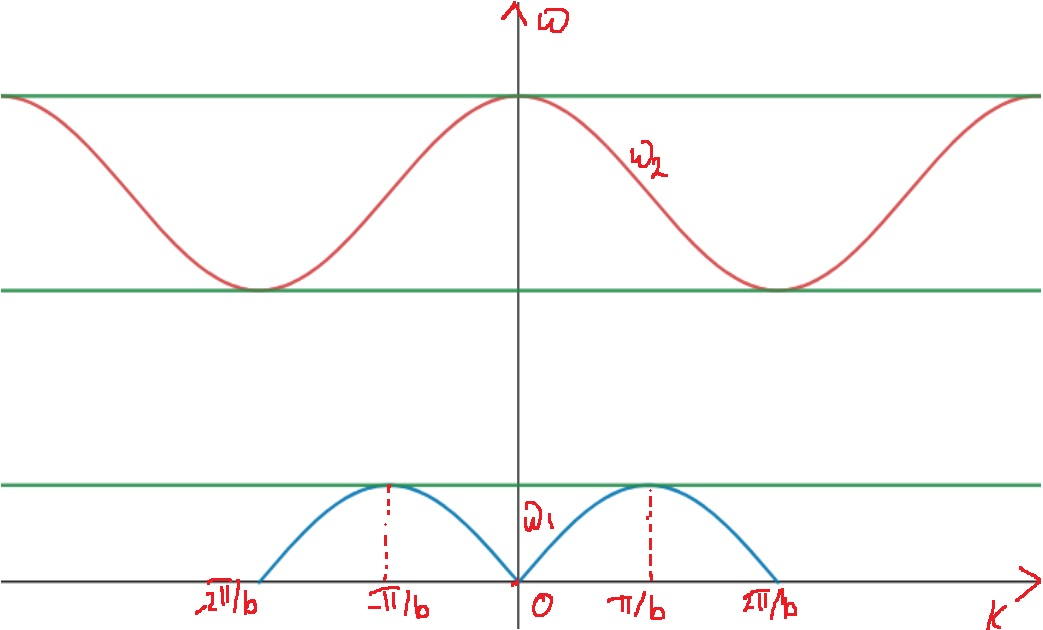
\includegraphics[width=90mm]{2.jpg}
\end{figure}
\end{frame}
\begin{frame}
	При малых k $\omega_1$ мала и изменяется линейно в зависимости k. В этом случае $\xi_0 = \eta_0$. 
	Поэтому располагаются на малых по сравнению с длиной волны отрезке.\newline
	$\omega_2$ при $k\to 0$ стремится к своему максимуму. Поэтому $M\xi_0 = -m\eta_0$. Следовательно соседние атомы колеблютя в противоположных фазах.
\end{frame} 

\end{document}
